\documentclass[10pt,twocolumn,letterpaper]{article}

\usepackage{cvpr}
\usepackage{times}
\usepackage{epsfig}
\usepackage{graphicx}
\usepackage{amsmath}
\usepackage{amssymb}
\usepackage{amsfonts}       % blackboard math symbols
%\usepackage{nicefrac}       % compact symbols for 1/2, etc.
%\usepackage{microtype}      % microtypography

\usepackage{url}
\usepackage[table]{xcolor}
\usepackage{bbm}
\usepackage{booktabs}
\usepackage[T1]{fontenc}
\usepackage{fix-cm}
\usepackage{array}
\usepackage{epsfig}
%\usepackage{mathabx}
%\usepackage{dsfont}
\usepackage{multirow}

\usepackage{times}
\usepackage{helvet}
\usepackage{courier}
\usepackage{graphicx}
\usepackage{bm}
\usepackage{color}
\usepackage{epstopdf}
\usepackage{caption}
\usepackage{subcaption}
\usepackage{enumitem}
\usepackage{calc}
\usepackage{multirow}
\usepackage{xspace}
\usepackage{booktabs}
\usepackage{mathrsfs}
\usepackage{array}
\usepackage{gensymb}

% Include other packages here, before hyperref.

% If you comment hyperref and then uncomment it, you should delete
% egpaper.aux before re-running latex.  (Or just hit 'q' on the first latex
% run, let it finish, and you should be clear).
\usepackage[pagebackref=true,breaklinks=true,letterpaper=true,colorlinks,bookmarks=false]{hyperref}

% \cvprfinalcopy % *** Uncomment this line for the final submission
\newcommand{\figref}[1]{Fig\onedot~\ref{#1}}
\newcommand{\equref}[1]{Eq\onedot~\eqref{#1}}
\newcommand{\secref}[1]{Sec\onedot~\ref{#1}}
\newcommand{\tabref}[1]{Tab\onedot~\ref{#1}}
\newcommand{\thmref}[1]{Theorem~\ref{#1}}
\newcommand{\prgref}[1]{Program~\ref{#1}}
\newcommand{\algref}[1]{Alg\onedot~\ref{#1}}
\newcommand{\clmref}[1]{Claim~\ref{#1}}
\newcommand{\lemref}[1]{Lemma~\ref{#1}}
\newcommand{\ptyref}[1]{Property\onedot~\ref{#1}}

\newcommand{\ve}[1]{{\mathbf #1}} % for displaying a vector or matrix
\newcommand{\hua}[1]{{\mathcal #1}}
\newcommand{\scr}[1]{{\mathcal #1}}
\newcommand{\by}[2]{\ensuremath{#1 \! \times \! #2}}

%\makeatletter
\DeclareRobustCommand\onedot{\futurelet\@let@token\@onedot}
\def\onedot{\ifx\@let@token.\else.\null\fi\xspace}
\def\eg{\emph{e.g.}}
\def\Eg{\emph{E.g}\onedot}
\def\any{\forall}
\def\ie{\emph{i.e.}}
\def\Ie{\emph{I.e}\onedot}
\def\cf{\emph{cf}\onedot}
\def\Cf{\emph{Cf}\onedot}
\def\etc{\emph{etc}\onedot}
\def\vs{\emph{vs}\onedot}
\def\wrt{w.r.t\onedot}
\def\dof{d.o.f\onedot}
\def\etal{\emph{et al.}}

\def\cvprPaperID{936} % *** Enter the CVPR Paper ID here
\def\httilde{\mbox{\tt\raisebox{-.5ex}{\symbol{126}}}}

% Pages are numbered in submission mode, and unnumbered in camera-ready
\ifcvprfinal\pagestyle{empty}\fi
\begin{document}

%%%%%%%%% TITLE
\title{DeepLocSeg: Online Camera Pose Estimation and Scene Parsing with Deep Learning and a 3D Semantic Map}

\maketitle
%\thispagestyle{empty}

%%%%%%%%% ABSTRACT
\begin{abstract}
Visual-based outdoor navigation requires accurately localizing the camera and preferably per-pixel semantic understanding, which can be widely applied for autonomous driving, or augment reality \etc.
%However, system solely relying on visual signal is non-robust due to visual confusion across multiple scenes.
%Thus, coarse signals from motion sensors, \eg GPS and IMU, are usually considered as a localization prior~\cite{}.
In this paper, we propose a deep learning based method for localizing the camera and parsing the recorded video simultaneously in a single framework, which fuses signals from camera and motion sensors like GPU and IOU.
Specifically in our setting, we have a 3D semantic world, and a video is recording online inside, meanwhile a non-accurate camera pose signal is observed.
In our system, at each timestamp, based on the obtained pose signal, we render a label map out of the 3D world, and feed it to a pose CNN jointly with the current frame of image, yielding a corrected camera pose.
Then, a multi-layer recurrent neural network (RNN) is performed afterwards, which captures high-order temporal information that further improve the pose accuracy.
Finally, based on the corrected pose from RNN, a new label map is rendered, and is fed into a segment CNN combining with the image, yielding a parsing of the scene.
In order to perform the experiments,  we build a dataset with a semantic labeled real world 3D map, jointly with many recorded videos with ground truth poses from high accurate motion sensors.
We show that practically, pose estimation solely relying on images like PoseNet~\cite{Kendall_2015_ICCV} may fail due to street view confusion, and it is important to fuse multi sensors. In addition, semantic parsing and pose estimation are mutually beneficial in learning more robust networks. Finally, various ablation studies are performed, which demonstrate the effectiveness of the proposed system.
\end{abstract}

%%%%%%%%% BODY TEXT
\section{Introduction}
\label{sec:introduction}
% the problem we are solving, distinguish with previous problems
In the applications like robotic navigation~\cite{ohno2003outdoor}, vision-based 6-DOF camera pose estimation~\cite{campbell2017globally,moreno2008pose,Kendall_2015_ICCV,coskun2017long} attracts much attention in computer vision.
Additionally, to acquire better scene understanding for applications such as augment reality~\cite{DBLP:journals/corr/abs-1708-05006}, parsing each frame of a video into semantically meaningful part is also important.

\begin{figure*}[t]
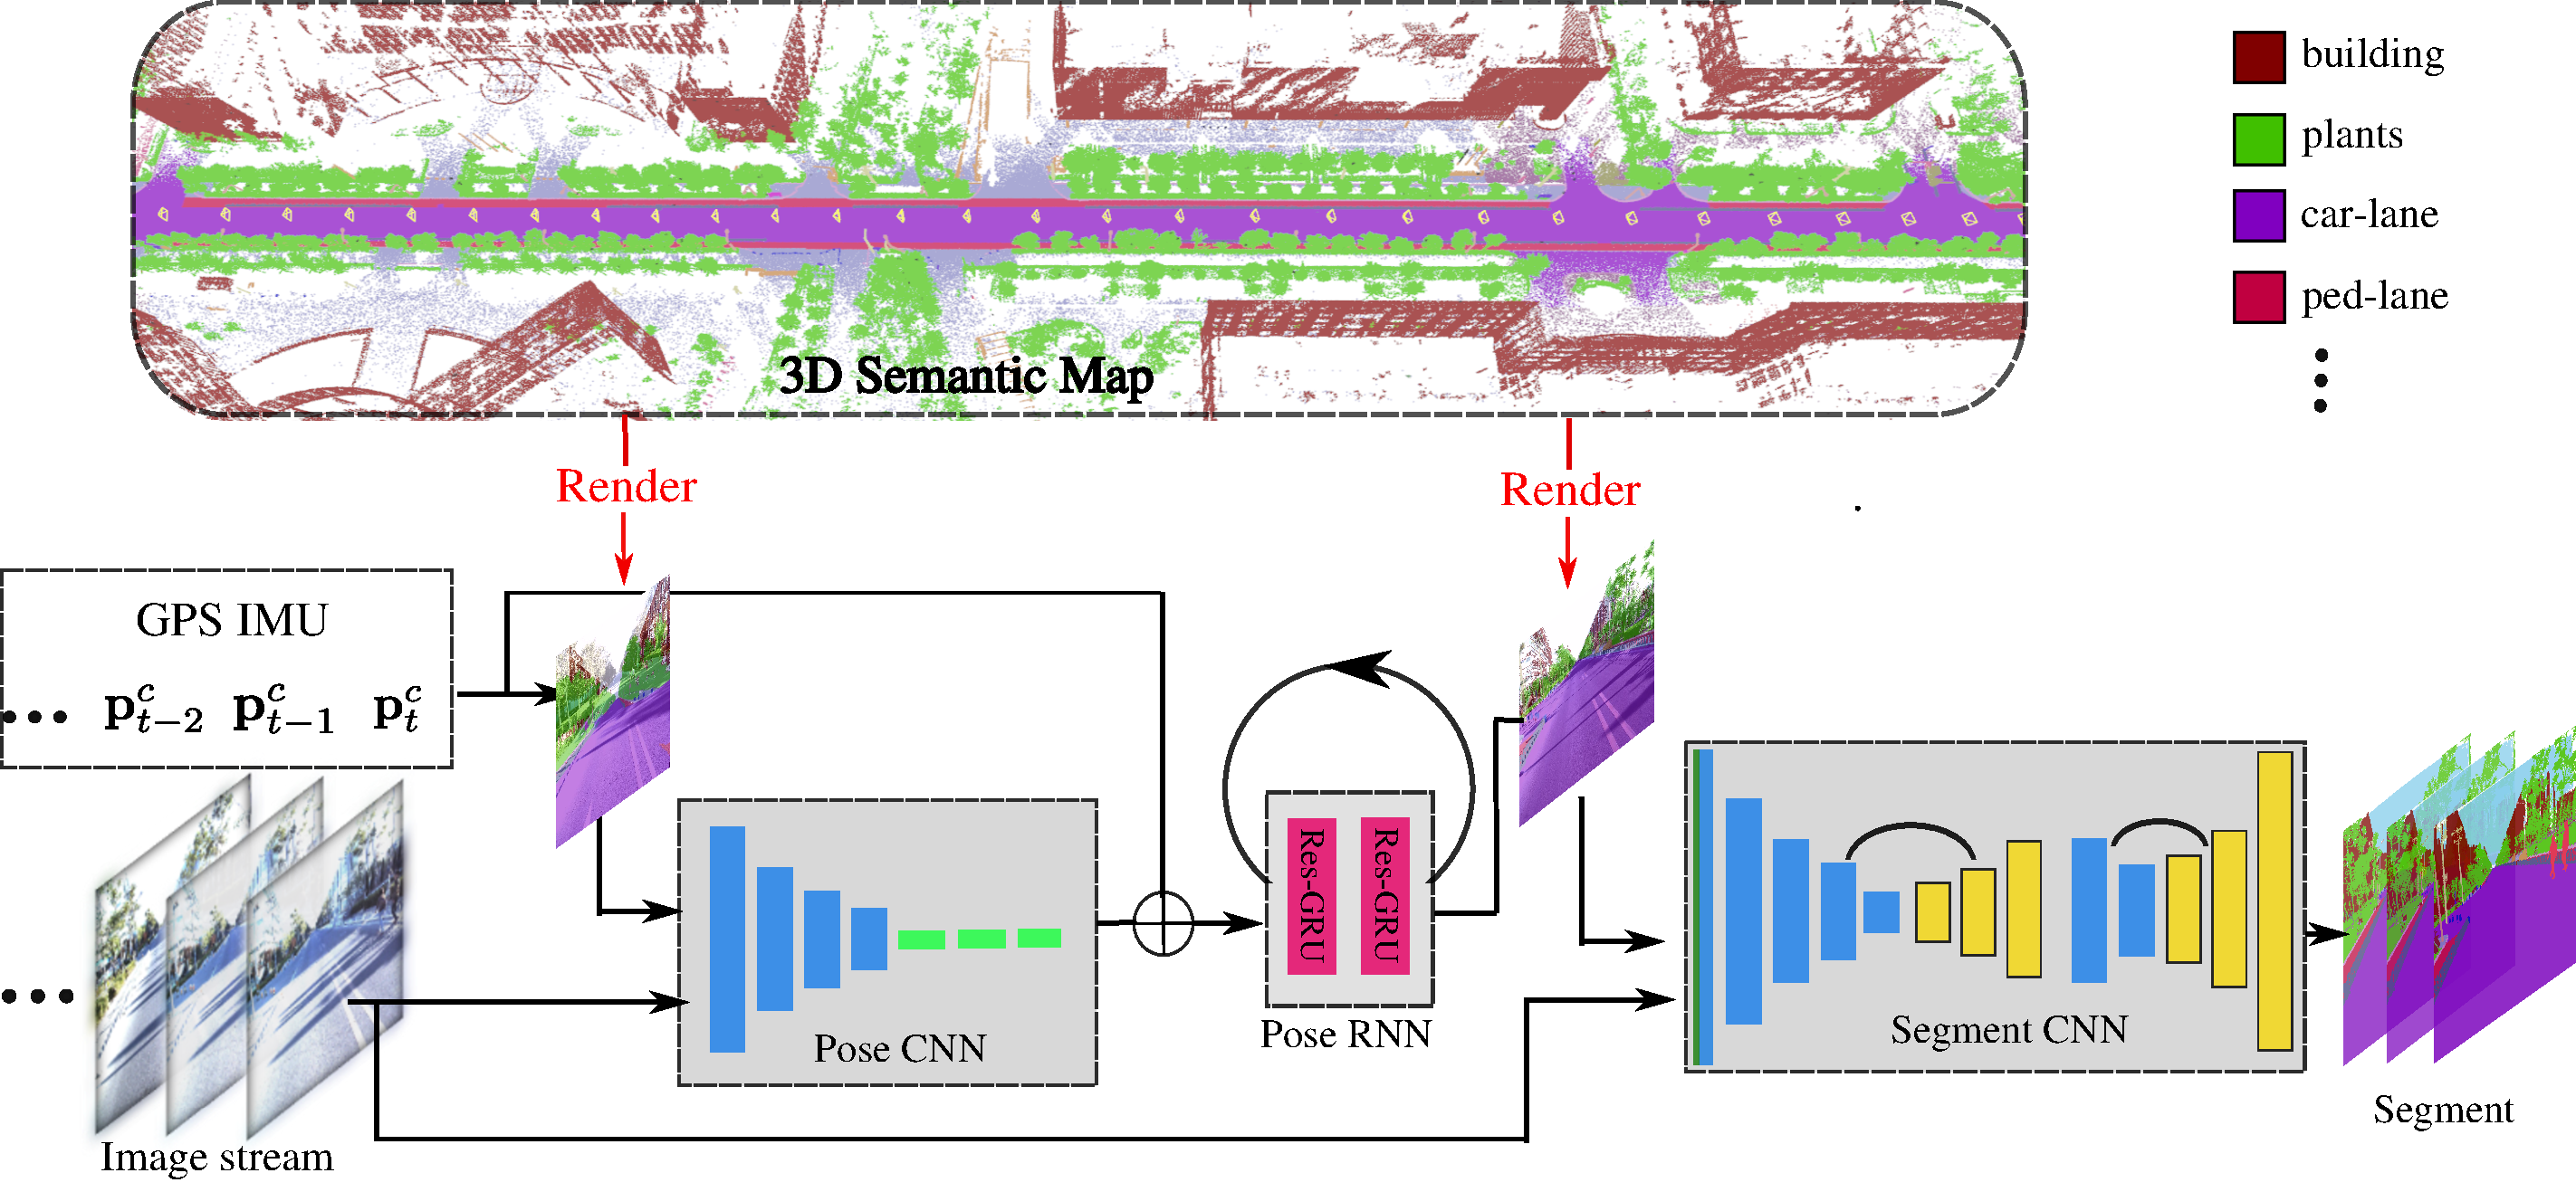
\includegraphics[width=\textwidth]{fig/framework.pdf}
\caption{System overview. The black arrows show the testing process, and red arrows indicate the rendering (projection) operation in training and inference. The yellow symbol shows the trajectory of the cameras.\textcolor{red}{check!} The input of our system contains a sequence of images and corresponding GPS/IMU signals. The outputs are the semantically segmented images, each with its refined poses.}
\label{fig:framework}
\end{figure*}

% existing methods only consider one of the tasks with soly visual signal.
Currently, most existing vision algorithms are trying to solve both tasks solely on visual signals.
For instances, geometric based methods are relying on visual feature matching, \eg~systems of Perspective-n-Points (PnP)~\cite{haralick1994review,kneip2014upnp,campbell2017globally} when a 3D map and an image is provided, or systems of SLAM~\cite{engel2014lsd,mur2015orb,NewcombeLD11} when there is a video. Such systems are relying on local appearance, which could fail when confronted with low-texture environments.

Most recently, deep learning based methods, \eg~for either images~\cite{Kendall_2015_ICCV} or videos~\cite{DBLP:journals/corr/ClarkWMTW17}, have been developed for real-time localization, which show good trade-offs between accuracy and speed.
Nevertheless, those methods are good for environments with rich distinguishable features, such as these in the Cambridge landmarks dataset~\cite{Kendall_2015_ICCV}. They could fail for common street views with very similar appearances or even repetitive structures.
%For example, when driving inside a tree-line street beside, can hardly localize the images without external signals.

For scene parsing, approaches~\cite{ZhaoSQWJ16,ChenPSA17} based on deep fully convolutional network (FCN) with ResNet~\cite{HeZRS15} are the better-performing algorithms for single image input. When the input is video, researchers~\cite{kundu2016feature,zhu2016deep} may incorporate the optical flow between consecutive frames, which not only accelerates the parsing, but also improve temporal consistency. Furthermore, for static background, one may use structure-from-motion (SFM) techniques~\cite{wu2011visualsfm} to jointly parse and reconstruct~\cite{kundu2014joint}. However, these methods can still be fragile in practice.

We aim to solve this camera localization and scene parsing problem from a more practical standpoint. That is, we assume that there will be (a) GPS/IMU signal to provide a rough location estimate; and (b) a semantic 3D map for the static environment. The GPS/IMU signal, even though noisy, serves as the crucial pose prior for our deep-learning based pose estimation system. The semantic 3D map, which could be rendered to a semantic label map for a given pose, not only provides strong priors for scene parsing, but also helps maintain temporal consistency.

%In our scenario, targeting at a more practical setting, we consider the video is online recorded, and a 3D semantic map is pre-built by us. For handling the localization confusion of street views, we propose to fuse signals from motion sensors like global positioning system (GPS) and inertial measurement unit (IMU), which is typically available for current navigation system. Those signals can be noisy but is crucial as a pose priori for our deep learning system.
%For video segmentation, we online render images from the 3D map, which serves as a priori for further segmentation, and helps the consistency along the temporal dimension.
%
In fact, our problem setting is on par with the widely used mobile navigation system, whereas the 2D labeled map is raise up to a 3D semantic map, and the problem of 2D location estimation is changed to 3D camera pose. Promisingly, with the accelerated development of autonomous driving, city-scale 3D semantic maps are being collected and built (such as the Toronto City dataset~\cite{wang2016torontocity}).  In our case, we constructed our own data with high quality 3D semantic map, which is captured by a high-accuracy mobile LIDAR device from $Riegl$\footnote{http://www.rieglusa.com/index.html}.

%lots of city scale 3D map has already collected from companies such as Google Earth~\cite{sheppard2009ethics} and Altizure\footnote{https://www.altizure.com/}, and also semantic labeled ones is also built such as Toronto city~\cite{wang2016torontocity}. In our case, we constructed our own data with high quality 3D semantic map, by adopting a high accuracy mobile LIDAR device from Riegl\footnote{http://www.rieglusa.com/index.html}.

Last but not least, within our deep learning framework, the camera pose and semantics are mutually beneficial, where pose helps establish the correspondences between the 3D semantic map and 2D semantic label map. Conversely, semantics could help refine camera poses. Our unified framework yields better results, in terms of both accuracy and speed, for both tasks than doing them individually. In our experiments, using a single core of Titan Z GPU, our system estimates the pose in 10ms with accuracy under 1 degree, and segments the image $512 \times 608$ in less than 100ms with pixel accuracy around 96$\%$, which demonstrates its efficiency and effectiveness.

% redefine our problem
In summary, the contributions of this paper are:
\begin{itemize}
    \item We propose a deep learning based system for fusing multiple information, \ie~camera images, GPS and IMU, and 3D maps, which helps to improve the robustness and accuracy for camera localization and scene parsing.
    \item Camera pose and scene semantics are handled jointly in both training and testing; they are mutually beneficial.
    \item We construct a dataset from real scenes to fully evaluate our approach. It includes dense 3D semantically labelled point cloud, ground truth camera poses and pixel-level segmentation of every frame, which we will release in order to benefit related research in computer vision.
\end{itemize}

The structure of this paper is organized as follows. We first give a overview of our system in \secref{sub:framework}. In \secref{sec:data_collection}, we first describe how our data is different from the existing outdoor datasets. In addition, we briefly introduce the method how the data is collect and labelled. Then, \secref{sec:localize_and_parsing} presents the framework and detail of our system. The full performance is evaluated quantitatively for both pose estimation and parsing in \secref{sec:experiments}, and \secref{sec:conclusion} concludes the paper and point out future directions. Finally, we will release all our code, models and dataset with the publication of this paper.


\subsection{Framework}
\label{sub:framework}
The framework of our system is illustrated in \figref{fig:framework}. At above, a pre-built 3D semantic map is available. During testing, an online stream of images and corresponding camera poses that is based on GPS/IMU are fed in to the system. Firstly, for each frame, a semantic label map is rendered out based on the input coarse camera pose. Then it is fed to a pose network jointly with the respective image.  The network calculates the relative rotation and translation, and yields a corrected camera pose. To build the temporal correlations, the corrected poses are fed into a RNN which further improves the pose accuracy in the stream.
Last, given the rectified camera pose, a new rendered label map is generated. We feed it together with the image to a segmentation network, which helps to segment a spatially more accurate and temporally more consistent result for the stream of video.
In this system, since our data contains ground truth for both pose and segments, it can be trained with strong supervision at each end of outputs.

\section{Related Work}
\label{sec:related_work}
Estimating camera pose and parsing images with a video or a single image have long been center problems for computer vision and robotics.
Here we summarize the related works in several aspects without enumerating all due to space limitation.
Notice that our driving application is autonomous driving,  we therefore focus on outdoor cases with street-level input. Localization and general parsing in the wild is beyond the scope of this paper.

% talk each perspective with image and video
\textbf{Camera pose estimation.} Traditionally, localizing an image given a set of 3D points is formulated as a Perspective-$n$-Point (P$n$P) problem~\cite{haralick1994review,kneip2014upnp} by matching feature points in 2D and features in 3D through cardinality maximization. Usually in a large environment, a pose prior is required in order to obtain good estimation~\cite{david2004softposit,moreno2008pose}. Campbell \etal~\cite{campbell2017globally} propose a global-optimal solver which leverage the prior. At the case that geo-tagged images are available, Sattler \etal~\cite{sattler2017large} propose to use image-retrieval to avoid matching large-scale point cloud.
When given a video, relative pose could be further modeled with methods like SLAM~\cite{engel2014lsd} etc, which increases the localization accuracy and speed.

Although these methods are effective in cases with distinguished feature points, they are still not practical for city-scale environment with billions of points, and they may also fail in areas with low texture, repeated structures, and occlusions.
Thus, recently, deep learned features with CNN is proposed to combine low-level and high-level feature for localization. PoseNet~\cite{Kendall_2015_ICCV,kendall2017geometric} takes an low-resolution image as input, which can estimate pose in 10ms \wrt a feature rich environment composed of distinguished landmarks. LSTM-PoseNet~\cite{hazirbasimage} further captures a global context after CNN features.
Given an video, later works incorporate Bi-Directional LSTM~\cite{DBLP:journals/corr/ClarkWMTW17} or Kalman filter LSTM~\cite{coskun2017long} to obtain better results with temporal information. However, in street-view scenario, considering a road with trees aside, in most cases, no significant landmark appears, which could fail the visual models. Thus, although noisy, signals from GPS/IMU are a must for localization in these cases~\cite{vishal2015accurate}, whereas the problem changes to estimating the relative pose between the camera view of a noisy pose and the real pose. To handle this, recently, Researchers ~\cite{laskar2017camera,ummenhofer2016demon} propose to concatenate two real images as a network input, while in our case, we concatenate the real image with online rendered label map from the noisy pose, which provides superior results in our experiments.

\textbf{Scene parsing.} For parsing a single image, most state-of-the-arts (SOTA) algorithms over street-view datasets like CityScapes~\cite{Cordts2016Cityscapes} are designed based on a FCN~\cite{WuSH16e} and a multi-scale context module with either dilated convolution~\cite{ChenPSA17}, pooling~\cite{ZhaoSQWJ16}, CRF~\cite{} or spatial RNN~\cite{byeon2015scene}. However, they are dependent on a ResNet~\cite{HeZRS15} with hundreds of layers, which is comparably too computationally expensive for applications that requires real-time performance. Some researchers apply small models~\cite{PaszkeCKC16} or model compression~\cite{ZhaoQSSJ17} for acceleration by sacrificing the accuracy.
When the input is a video, spatial-temporal graph is built, Kundu \etal~\cite{kundu2016feature} use 3D dense CRF to get temporal consistent results. Recently, optical flow~\cite{dosovitskiy2015flownet} between consecutive frames is computed to transfer label or features~\cite{gadde2017semantic,zhu2016deep} from the previous frame to the current one.  Significant progress has been made, yet the consistency is built through flow, rather than 3D information and camera pose, which is more compact to use. In our case, we use the rendered label map from 3D as the prior to the segment network, which leverage the difficulty of scene parsing solely from image cue. For practicality, we also adopt the light weighted network from DeMoN~\cite{ummenhofer2016demon} to keep the system consistent \textcolor[rgb]{1.00,0.00,0.00}{of what?}.


\textbf{Joint 2D-3D for video parsing.} Another set of works that could be related with ours is joint reconstruction, pose estimation and parsing~\cite{kundu2014joint,hane2013joint} through 2D-3D consistency supervised training.
 Traditionally, those methods are reliant on structure-from-motion (SFM)~\cite{hane2013joint} from feature or photometric matching. Specifically, they reconstruct a 3D map and performing semantic parsing over 2D and 3D jointly, yielding consistent segmentation between multiple frames.
 Most recently, CNN-SLAM~\cite{tateno2017cnn} replaces the 3D reconstruction using a depth network from a single image, and a segment network for image parsing.
 However, all there approaches are processed off-line and only for static background, which does not satisfy our online setting. Moreover, the quality of reconstructed 3D model is not comparable with the one directly collected from real world. \textcolor[rgb]{1.00,0.00,0.00}{you mean our scanner?}
% traditional key points, slam etc
% pnp
% marc's paper
% hongdong's paper
% silvio's paper
% posenet related
% jifeng's paper
% iccv kalman
% domain transfer etc
\section{Dataset Preparation}
\label{sec:data_collection}
\begin{table*}[t]
\center
\begin{tabular}{lccccc}
\toprule[0.2 em]
% \thickhline
Dataset & Real data & Camera pose & 3D map & Video per-frame labeling  & Temporal variations  \\
\hline
\multicolumn{1}{l|}{CamVid~\cite{brostow2009semantic}}     &\checkmark                       & -              & -              &  -  & -  \\
\multicolumn{1}{l|}{KITTI~\cite{geiger2012we}}      &\checkmark  & \checkmark     & sparse points  & -   & -  \\
\multicolumn{1}{l|}{CityScapes~\cite{Cordts2016Cityscapes}} &\checkmark  & -              &  -             & selected frames & - \\
\multicolumn{1}{l|}{Toronto~\cite{wang2016torontocity}}    &\checkmark  & \checkmark     & sparse points  & selected pixels & - \\
\hline
\multicolumn{1}{l|}{Synthia~\cite{RosCVPR16}}    & -          & \checkmark     & -       &\checkmark & -    \\
\multicolumn{1}{l|}{Play for benchmark~\cite{richter2017playing}} &-   & \checkmark     & -     &\checkmark & - \\
\hline
\multicolumn{1}{l|}{Ours}              & \checkmark &\checkmark    &dense point cloud  & \checkmark     &  \checkmark \\
\toprule[0.2 em]
\end{tabular}
\caption{Compare our data with the other related outdoor street-view datasets for our task. 'Real data' mean whether the data is collected from realistic world.
'3D map' means whether it contains 3D map of the whole dataset. 'Video per-frame labeling' means whether it has per-frame per-pixel semantic label.
'Temporal variations' mean whether the recorded video can roughly cover the whole scene, but have multiple. \textcolor[rgb]{1.00,0.00,0.00}{we don't have temporal varations here, we didn't present results on this point neither, that last column needs to be removed. I would also argue the Toronto one is good. 
it has 3D model, so it is dense. In the scope of this paper, we want to paint the picture that 3D maps will be available, so we don't want to over-sell the  uniqueness of our data set.  }}
\label{tbl:data}
\vspace{-0.3\baselineskip}
\end{table*}

\paragraph{Motivation.}
As described in the \secref{sub:framework}, our system is performed with available motion sensors and a semantic 3D map.
However, similar outdoor dataset produced by prior arts such as KITTI and CityScapes, does not containing such information, in particular the 3D map. The Tortoro City dataset~\cite{wang2016torontocity} could be used. However, it is not open yet. As summarized in \tabref{tbl:data}, we list several key properties to perform our experiments.
As can be seen, existing ones that are already open do not satisfy our requirements, especially for pose estimation, 

\textcolor[rgb]{1.00,0.00,0.00}{as I explained in the table, I suggest that we drop this argument, we need to have a 3D semantic map, none has it. the temporal effect needs to be tuned down, otherwise, it will be viewed as too narraow}
for training, we want the recorded video to roughly cover the 3D environment, so that when new images come in, appearance similar views had been seen during training. This means repeated recording at similar spatial locations are required in the data, which we call temporal variations in \tabref{tbl:data}.
However, most existing datasets are a temporal snapshot at some locations in the environment, which requires us to collect a new dataset ourselves.

\paragraph{Data collection.}
We use a mobile LIDAR scanner from $Riegl$ to collect point clouds of the static 3D map with high granularity. As shown in \figref{fig:data}(a). The captured point cloud density is much higher than the Velodyne\footnote{http://www.velodynelidar.com/} used by KITTI~\cite{geiger2012we}.
% Amazingly, it is even able to capture the hight changes of curb on road.
However, different from the sparse Velodyne LIDAR, our mobile scanner utilizes a single laser beam to scan a vertical circle. As the scanner moves, it is able to scan its surroundings as a push-broom camera. It cannot correctly capture moving objects, they will be compressed or expanded or completely missing in the resulting point cloud.
In order to remove those fake object points, thanks to the fact that the 3D world is recorded multiple rounds, and each round has a full coverage of the 3D map, we can use point clouds consistency to handle the issue.
Specifically, we calibrate the 3D point clouds from different rounds, and put all the points together. From the merged point cloud, the points with high temporal consistency from other rounds are kept, while those with low consistency are removed. Formally, the condition to kept a point $\ve{x}$ in round $j$ is,
\begin{align}
\sum_{i=0}^{r}{\mathbbm{1}(\exists~\|\ve{x}_i - \ve{x}_j\| < \epsilon_d )} / r \geq \delta
\end{align}
where $\delta = 0.7$ and $\epsilon_d = 0.025$ in our experiments, and $\mathbb{1}()$ is a indicator function. Notice due to the symmetric property of $\ve{x}_i$ and $\ve{x}_j$, we obtain the static points for all rounds by looping over the points of a single round. We keep the merged point cloud as a static background $\hua{M}$ for further labelling.

For video, we use two cameras facing towards direction of street with a resolution of \by{2048, 2432}, and both cameras are well calibrated \wrt the LIDAR. Based on provided camera parameters from the hardware, all the images from videos are undistorted to match the 3D points.
% talk about registration and removing moving objects inside data

% Undistortion of the image
\paragraph{Label 3D map and videos.}
% talk about labelling in 3D
In order to have semantic labelling of each frame in video, we handle static background, static objects and moving objects separately.
Firstly, for static background, we directly perform labelling on the 3D point cloud $\hua{M}$ which is then projected to images, yielding labelled background for all the frames.
Specifically, we over-segment the point cloud data into point clusters based on spatial distance and normal directions, and then we ask labellers to label each cluster of points manually.
For static objects in each round of video, we prune out the points of static background, and label the remaining points of objects. Due to the fact that when object is static, \eg parked cars, the shape and location of captured points will be highly recognizable, whereas when the object is moving on the road, the points will be fuzzy, we ask labeller to label those can be well recognized as static objects. Last, after projecting the 3D to 2D, only moving objects remain to be labeled. Here, we adopt an active labelling strategy, by first training an object segmentation model using a SOTA algorithm~\cite{WuSH16e}, and ask labellers to correct and label the masks of moving objects.

Finally, as shown in \figref{fig:data}(c), the projected label from 3D points is not perfect, due to missing points either too far away or reflection. We handle such issue by using splatting techniques in computer graphics, that is to turn each point into a small squaure as discussed in \secref{sub:render} (\figref{fig:data}(d)), and then ask labeller to fix missing regions, yielding the final label map (\figref{fig:data}(e)).
With such a strategy, labelling efficiency of video can be vastly increased, avoiding labelling edge rich regions like trees and poles on the street, especially when occlusion is happened.
We provided the labelled video in our supplementary materials for readers who are interested.

\begin{figure}[t]
\begin{center}
\fbox{\rule{0pt}{2in} \rule{0.9\linewidth}{0pt}}
\end{center}
   \caption{Snapshot of our collected data. (a) 3D semantic map. (b) Images. (c) Rendered label map with 3D points (d) Rendered label map with enlarged square. (e) Merge label map with object and sky.}
\label{fig:data}
\end{figure}


\vspace{-0.5\baselineskip}
\section{Localizing camera and scene parsing.}
\vspace{-0.3\baselineskip}
\label{sec:localize_and_parsing}
As shown in \secref{sub:framework}, our full system is based on a semantic 3D map and deep networks. In the following, we will first describe how a semantic label map is rendered from the 3D, then discuss the details of our network architectures and the loss functions to train the whole system.

\subsection{Render a label map from a camera pose.}
\label{sub:render}
Formally, given a 6-DOF camera pose $\ve{p} = [\ve{q}, \ve{t}] \in SE(3)$, where $\ve{q} \in SO(3)$ is the quaternion representation of rotation and $\ve{t} \in \mathbbm{R}^3$ is translation, a label map can be rendered from the semantic 3D map, where z-buffer is applied to find the closest point at each pixel.

In our setting, the 3D map is a point cloud based environment. Although the density of the point cloud is very high (one point per 25mm within road regions), when the 3D points are far away from the camera, the projected points could be sparse, \eg regions of buildings shown in \figref{fig:data}(c).
Thus for each point in the environment, we adopt the splatting technique in computer graphics, by enlarging the 3D point to a square where the square size is determined by its semantic class. Formally, for a 3D point $\ve{x}$ belonging a class $c$, its square size $s_c$ is set to be proportional to the class' average distance to the camera. Formally,
{\vspace{-0.3\baselineskip}
\begin{align}
\label{eq:square_size}
s_c \propto \frac{1}{|\hua{P}_c|}\sum_{\ve{x}\in \hua{P}_c} \min_{\ve{t}\in\hua{T}} d(\ve{x}, \ve{t})
\end{align}
}
where $\hua{P}_c$ is the set of 3D points belong to class $c$, and $\hua{T}$ is the set of ground truth camera poses. Then, given the relative square size between different classes, in order to obtain the absolute size for rendering, we have to define an absolute range. This is non-trivial since too large size will result in dilated edges, while too small size will yield many holes. In our experiments, we set the range as $[0.025, 0.05]$, and found it provide the highest visual quality.

As shown in \figref{fig:data}(e), invalid values in-between those projected points are well in-painted, meanwhile the boundaries separating different semantic classes are also well preserved. Later, we insert such a rendered label map for the pose CNN, which guides the network to localize the camera.
% By feeding in such a rendered map, it facilitates the CNN to better discover scene layouts both for pose estimation and scene parsing.
% Another possibility is to render a RGB image rather than a label map. However, we found label map works better, which may be due to it contains less noisy edges than rendered RGB image. \textcolor{red}{it is not certain, should we even bother to say it?}
% AOne may wonder why we render semantic label map rather than synthesizing a RGB image for later inputs.
% This is because intuitively label maps is invariant to color changes, which yields better boundaries reflecting the scene layout.

\begin{figure}[t]
\begin{center}
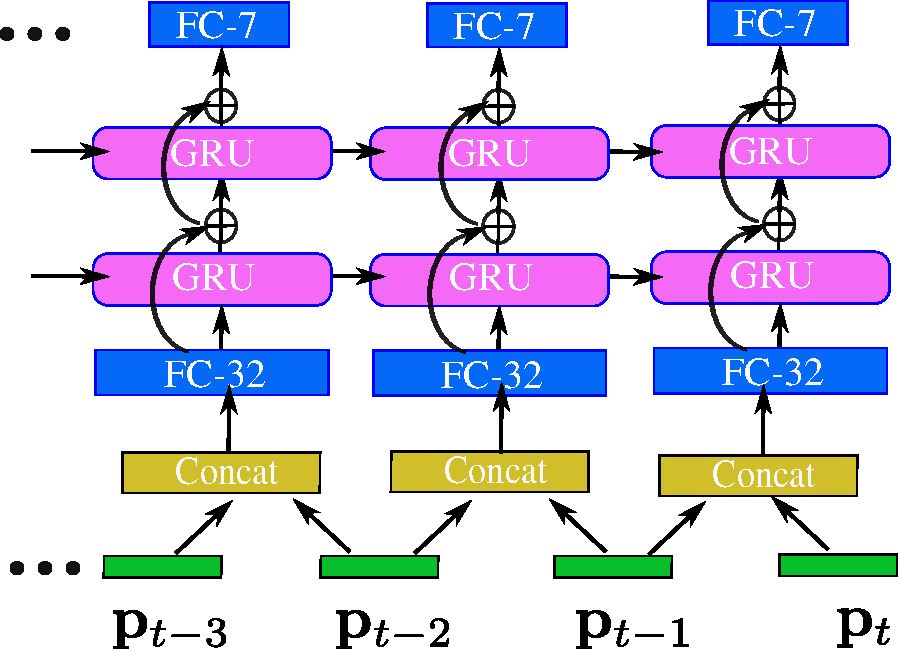
\includegraphics[width=.8\linewidth]{fig/RNN.pdf}
\end{center}
   \caption{The GRU RNN network architecture for modeling a sequence of camera poses.}
\label{fig:rnn}
\vspace{-1.1\baselineskip}
\end{figure}

\vspace{-0.3\baselineskip}
\subsection{Camera localization with motion prior}
\vspace{-0.2\baselineskip}

\textbf{Translation rectification with road prior.} One common localization priori for navigation is to use the 2D road map, by constraining the GPS signals inside the road regions. We adopt a similar strategy, since once the GPS signal is out of road regions, the rendered label map will be totally different from the street-view of camera, and no correspondence can be found by the network.

To implement this constraint, firstly we can render a 2D road map image with a rasterization grid of $0.05m$ from our 3D semantic map by using only road points, \ie points belong to car-lane, pedestrian-lane and bike-lane \etc
Then, at each pixel $[x, y] \in \mathbbm{Z}^2$ in the 2D map, an offset value $\ve{f}(x, y)$ is pre-calculated indicating its 2D offset to the closest pixel belongs to road. We can calculate $\ve{f}()$ very efficiently with a breath-first-search algorithm.

During online testing, given a noisy translation $\ve{t}=[t_x, t_y, t_z]$, we can find the closest road points \wrt $\ve{t}$ using $[t_x, t_y] + \ve{f}(\lfloor t_x \rfloor, \lfloor t_y \rfloor)$ from our pre-calculated offset function. Then, a label map is rendered based on the rectified camera pose, which is later fed to pose networks.

\begin{figure*}[t]
\center
\vspace{-0.6\baselineskip}
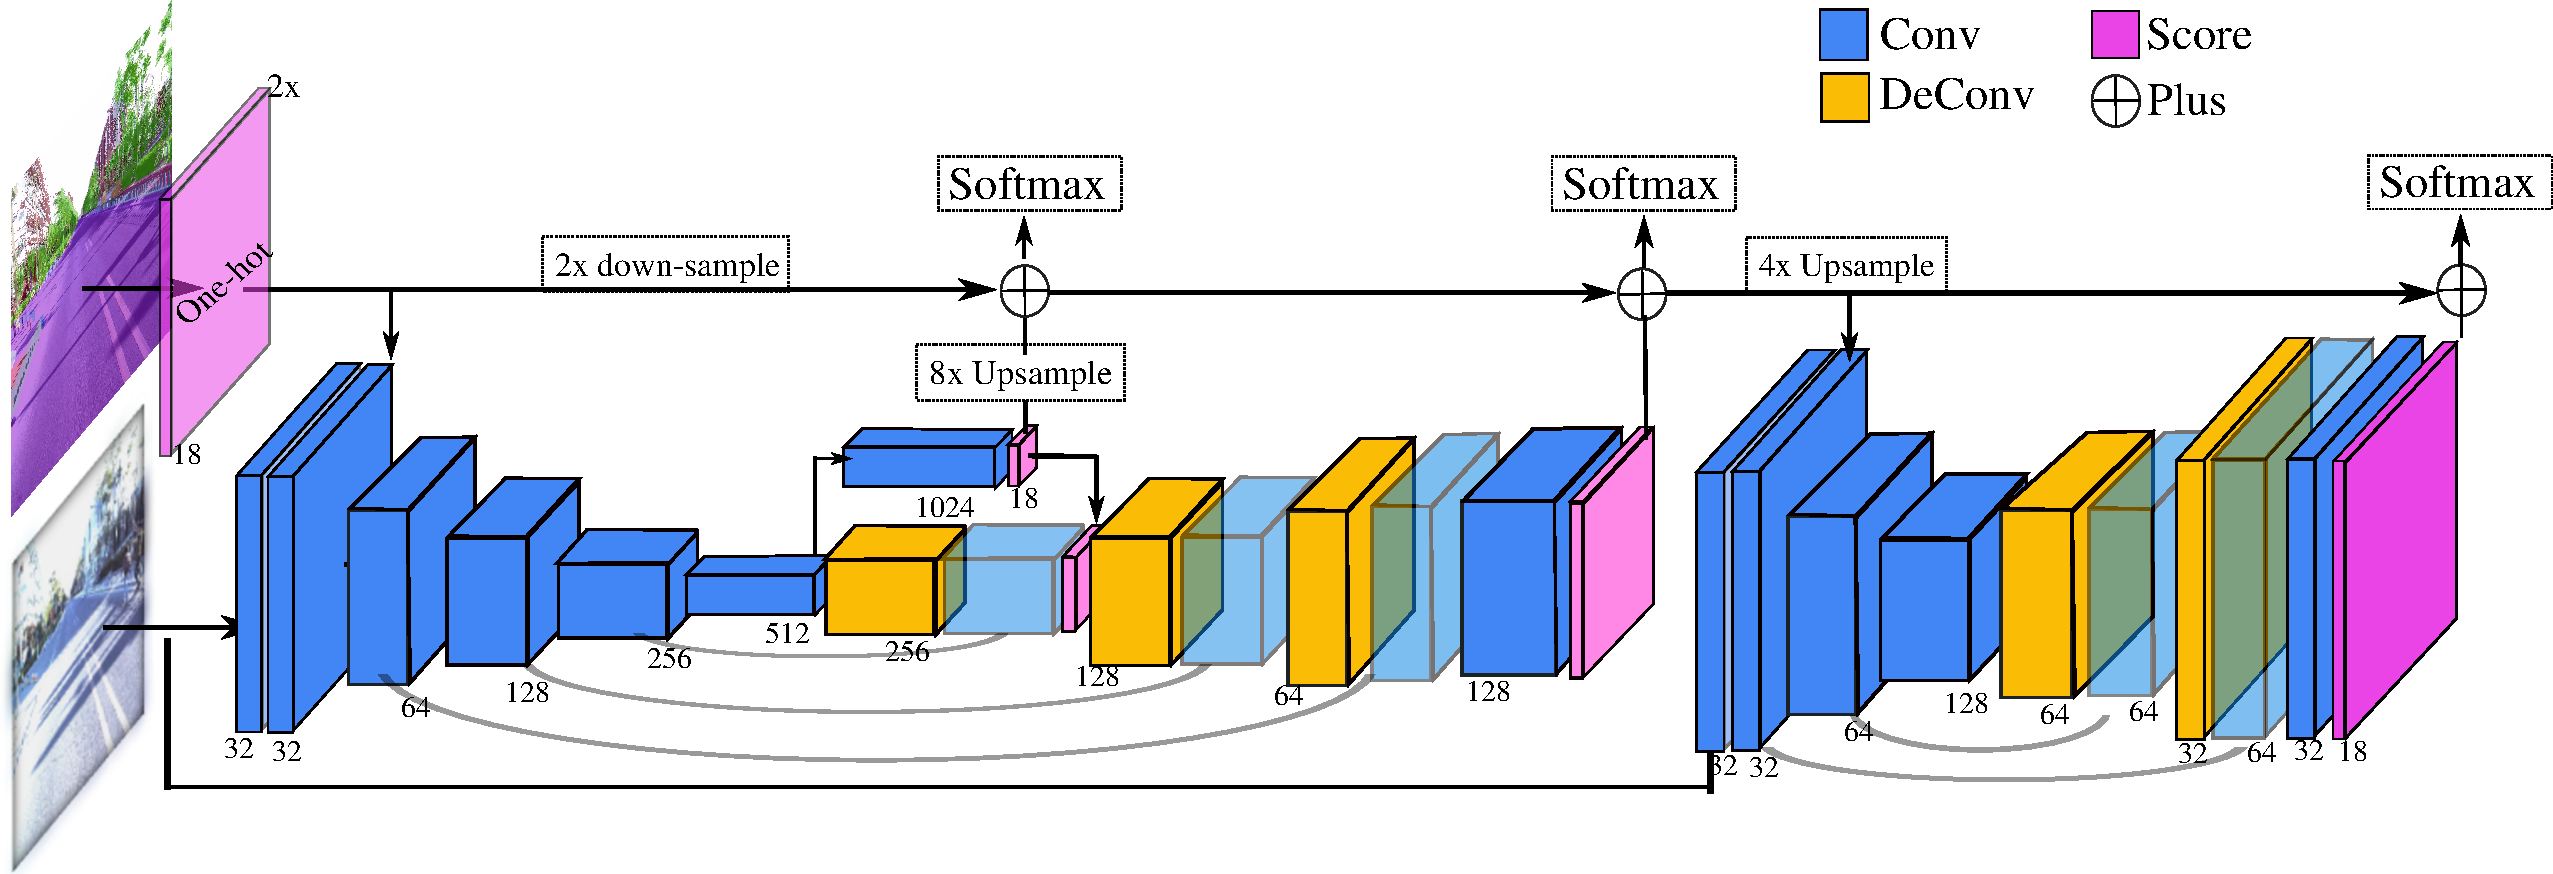
\includegraphics[width=0.95\textwidth]{fig/segCNN.pdf}
\caption{Architecture of the segment CNN with rendered label map as a segmentation priori. At bottom of each convolutional block, we show the filter size, and at top we mark the downsample rates of each block \wrt the input image size. The 'softmax' text box indicates the places a loss is calculated. Details are in \secref{subsec:parsing}.}
\label{fig:segnet}
\vspace{-1.2\baselineskip}
\end{figure*}
\textbf{CNN-GRU pose network architecture.}
As shown in \figref{fig:framework}, our pose networks contain a pose CNN and a pose GRU-RNN. Particularly,
the CNN of our pose network takes as inputs an image $\ve{I}$ and the rendered label map $\ve{L}$ from corresponding coarse camera pose $\ve{p}_i^c$. It outputs a 7 dimension vector $\hat{\ve{p}}_i$ representing the relative pose between the image and rendered label map, and we can get the pose \wrt the 3D map by $\ve{p}_i = \ve{p}_i^c + \hat{\ve{p}_i}$.
For the network architecture of pose CNN, in order to have large kernel to obtain bigger context while keeping the amount of parameters and runtime manageable, we follow the design of DeMoN~\cite{ummenhofer2016demon}. The convolutional kernel of this network consists a pair of 1D filters in $y$ and $x$-direction, and the encoder gradually reduces the spatial resolution with stride of 2 while increasing the number of channels. We list the details of the network in our implementation details at \secref{sec:experiments}.

Additionally, since the input is a stream of images, in order to model the temporal dependency,
after the pose CNN, a multi-layer GRU with residual connection~\cite{wu2016google} is appended.
More specifically, we adopt a two layer GRU with 32 hidden states as illustrated in \figref{fig:rnn}, which includes high order interaction beyond nearby frames, which is sufficient for improve the pose estimation performance.
In traditional navigation applications of estimating 2D poses,  Kalman filter~\cite{kalman1960new} is commonly applied by assuming either a constant velocity or acceleration.
In our case, due to the speed of vehicle is unknown, transition of camera poses is learned from the training sequences, and in our experiments we show that the motion predicted from RNN is better than using a Kalman filter with a constant of speed, yielding further improvement over the estimated ones from our pose CNN.

\textbf{Pose loss.}
Following the PoseNet~\cite{kendall2017geometric}, we use the geometric matching loss for training, which avoids the balancing factor between rotation and translation.
Formally, given a set of point cloud in 3D $~\hua{P}=\{\ve{x}\}$, and the loss for each image is written as,
{\vspace{-0.5\baselineskip}
\begin{align}
L(\ve{p}, \ve{p}^*) = \sum_{\ve{x} \in \hua{P}}\omega_{l_\ve{x}}|\pi(\ve{x}, \ve{p}) - \pi(\ve{x}, \ve{p}^*)|_2
\label{eq:proj_loss}
\end{align}
}
where $\ve{p}$ and $\ve{p}^*$ are the estimated pose and ground truth pose respectively. $\pi()$ is a projective function that maps a 3D point $\ve{x}$ to 2D image coordinates. $l_\ve{x}$ is the semantic label of $\ve{x}$ and $\omega_{l_\ve{x}}$ is a weight factor dependent on the semantics. Here, we set stronger weights for point cloud belong to certain classes like traffic light, and we find it helps pose CNN to achieve better performance.
In~\cite{kendall2017geometric}, usually the 3D points visible to the camera are used by this loss to avoid very large numbers and ensure the stableness of training. However, online searching the visible 3D points from millions is not practical.
Thus, we pre-render a depth map for each training image with a resolution of $256 \times 304$, based on its ground truth pose, and use the back projected 3D points from the depth map for training.

% Intuitively, we find the amount of points in each class is dramatically unbalanced, and most points are those on roads and trees. Nevertheless, the appearance variation of road and trees are not very sensitive to pose changes in the street-view scenario. In order to encourage the network to discover more str
% Thus,  other structures images like electricity pole or road light have rich structures like edges and textures, which potentially should be valued more for matching.
% In~\cite{ummenhofer2016demon}, the model try to predict a flow confidence map revealing the texture rich regions which helps pose estimation. In our work, we adopt the labelled semantic labels, and reweight each 3D point in the training loss, which drives the network to focus more on
% Thus, the learning loss changed to
% \begin{align}
% L(\ve{p}, \ve{p}^*) = \sum_{\ve{x} \in \hua{P}}\omega_{l_\ve{x}}|\pi(\ve{x}, \ve{p}) - \pi(\ve{x}, \ve{p}^*)|_2
% \label{eq:proj_loss}
% \end{align}
% where $\omega_{l_\ve{x}}$ is the weight of class $l_\ve{x}$. We set the weight for each class depends on the class edgeness which is the percentage of pixel along the edge
\subsection{Video parsing with pose guidance}
\label{subsec:parsing}
Having rectified pose at hand, one may direct render the semantic 3D world to the view of a camera, yielding a semantic parsing of the current image. However, the estimated pose is not perfect, fine regions such as light poles can be completely misaligned. Other issues also exist. Many 3D points are missing due to reflection, \eg regions of glasses, and points can be sparse at long distance. Last, dynamic objects in the input cannot be represented by the projected label map, yielding incorrect labelling. Thus, we propose an additional segment CNN to tackle these issues, while taking the rendered label map as segment priori.
% In our experiments, we show with pose rendered label map as an additional input, the segment results are temporally more consistent and yields better accuracy.

\textbf{Segment network architecture.} As discussed in \secref{sec:related_work}, heavily parameterized networks such as ResNet are not efficient enough for our online application. Thus, as illustrated in \figref{fig:segnet}, our segment CNN is a light-weight network containing an encoder-decoder network and a refinement network, and both have similar architecture with the corresponding ones used in DeMoN~\cite{ummenhofer2016demon} including 1D filters and mirror connections. However, since we have a segment prior from the 3D semantic map, we add a residual stream (top part of \figref{fig:segnet}), which encourages the network to learn the differences between the priori map with the ground truth. In~\cite{pohlen2016full}, a full resolution stream is used to keep spatial details, while here, the rendered label map also helps to keep the semantic spatial layout.

Another notable difference for encoder-decoder network from DeMoN is that for network inputs, shown in \figref{fig:segnet}, rather than directly concatenate the label map with input image, we first transform the label map to a score map through one-hot operation, and embed the score of each pixel to a 32 dimensional feature vector. 
% This is to balance the two.\textcolor{red}{not very clear here, how is this balanced?} 
Then, we concatenate this feature vector with the first layer output from image, where the input channel imbalance between image and label map is alleviated for segmentation, which is shown to be useful by previous works~\cite{eigen2015predicting}.
 For refinement network, we use the same strategy to handle the two inputs. Finally, the segment network produces a score map, yielding the semantic parsing of the given image.

We train the segment network first with only RGB images, then fine-tune the network by adding the input of rendered label maps. This is because our network is trained from scratch, therefore it needs a large amount of data to learn effective features from images. However, the rendered label map from the estimated pose has on average 70$\%$ pixel accuracy, leaving only 30$\%$ of pixels having effective gradients. This could easily drive the network to over fit to the input label map, while slowing down the process towards learning features from images. Finally, for segmentation loss, we use the standard softmax loss, and add intermediate supervision right after the outputs from both the encoder and the decoder as indicated in \figref{fig:segnet}. 
\vspace{-0.1\baselineskip}
\section{Experiments}
\vspace{-0.1\baselineskip}
\label{sec:experiments}
We perform all experiments using our collected dataset, and evaluate multiple system settings for pose and segment to validate each component.
For obtaining GPS and IMU signal, due to at each time step, only one sampled noisy signal can obtained. This is limited for training the system. Thus, follow~\cite{vishal2015accurate}, we simulate noisy GPS and IMU by adding random perturbation $\epsilon$ \wrt ground truth pose following uniform distributions. 
Specifically, translation and rotation noise are set as $\epsilon_t \sim U(0, 7.5m)$ and $\epsilon_r \sim U(0^{\circ}, 15^{\circ})$ respectively. 
We refer to realistic data~\cite{lee2015gps} for setting the noisy range of simulation.

In this paper, our data vehicle collected 6 videos at different daytimes surrounding a technology park. The 3D map generated in our experiment has a road length around 3500$m$, and the distance between consecutive frames is around 5$m$ to 10$m$. We use 4 of the videos for training and 2 for testing, yielding 2242 training images and 756 testing images. The semantic classes, as shown in \figref{fig:data}, include $\{$sky, car-lane, pedestrian-lane, bike-lane, curb, traffic-cone, traffic-stack, traffic-fence, light-pole, traffic-light, tele-pole, traffic-sign, billboard, building, security-stand, plants, object $\}$. In the future, we are targeting at constructing even larger datasets with more semantics.

\textbf{Implementation details.} To quickly render from the 3D map, we adopt OpenGL to efficiently render a label map with the z-buffer handling. A 512 $\times$ 608 image can be generated in 70ms with a single Titan Z GPU, which is also the input size for both pose CNN and segment CNN. 
For pose CNN, the filter size of each layers is $\{32, 32, 64, 128, 256, 1024, 128, 7\}$, and the forward speed for each frame is 9ms. For pose RNN, we sample sequences with length of 100 from our data for training, and on average is cost 0.9ms for each frame.
For segment CNN, we keep the size the same as input, and the forward times is 90ms. 
Both of the network is learned with 'Nadam' optimizer~\cite{dozat2016incorporating} with a learning rate $10^{-3}$. We sequentially train the three models due to GPU memory limitation.
Specifically, for pose CNN and segment CNN, we stops at 150 epochs when there is no performance gain, and for pose RNN, we stops at 200 epochs. For data augmentation, we use the imgaug\footnote{https://github.com/aleju/imgaug} library to variate lighting, blurring and flipping. We select a subset from training images for validating the trained model from each epoch, and choose the model performing best for evaluation.

For testing, since input GPS/IMU contains variations, \ie~$\ve{p}_t^c=\ve{p}^*+\epsilon$, we need to have a confidence range of prediction for both camera pose and image segment, in order to verify the improvement of each component we have is significant. Specifically, we report the standard variation of the results from a 10 time simulation to obtain the confidence range. Finally, we implement all the networks by adopting the MXNet~\cite{ChenLLLWWXXZZ15} platform.

For pose evaluation, we use the median translation offset and median relative angle~\cite{Kendall_2015_ICCV}. For evaluating segment, we adopt the commonly use pixel accuracy (Pix. Acc.), mean class accuracy (mAcc.) and mean intersect-over-union (mIOU) as that from~\cite{WuSH16e}.

\begin{table}
\vspace{-0\baselineskip}
\center
\fontsize{7}{8}\selectfont
\hspace*{-0.33cm}
\begin{tabular}{llll}
\toprule[0.1 em]
% \thickhline
Method & Trans (m) $\downarrow$ & Rot ($\circ$)$\downarrow$  & Pix. Acc($\%$)$\uparrow$ \\
\hline
PoseNet~\cite{kendall2017geometric} & -  & -  & -  \\
Noisy pose & 3.45 $\pm$ 0.176 & 7.87 $\pm$ 1.10 & 54.01 $\pm$ 1.5 \\
Pose CNN w/o semantic & 1.355 $\pm$ 0.052  & 0.982 $\pm$ 0.023 & 70.99 $\pm$ 0.18 \\
Pose CNN w semantic & 1.331 $\pm$ 0.057  & 0.727 $\pm$ 0.018 & 71.73 $\pm$ 0.18  \\
Pose RNN w/o CNN & 1.282 $\pm$ 0.061  & 1.731 $\pm$ 0.06 &  68.10 $\pm$ 0.32 \\
Pose CNN w KF & 1.281 $\pm$ 0.06  & 0.833 $\pm$ 0.03 & 72.00 $\pm$ 0.17  \\
Pose CNN-RNN  & \textbf{1.005} $\pm$ 0.044  & \textbf{0.719} $\pm$ 0.035  & \textbf{73.01} $\pm$ 0.16  \\
\toprule[0.1 em]
\end{tabular}
\caption{Compare the accuracy of different settings for pose estimation.
Noisy pose indicates the noisy input signal from GPS, IMU, and 'KF' means kalman filter.
The number after $\pm$ indicates the std from 10 simulations. $\downarrow \& \uparrow$ means lower the better and higher the better respectively. 
We can see the improvement is statistically significant.}
\label{tbl:pose}
\vspace{-1.5\baselineskip}
\end{table}

\textbf{Pose Evaluation.}
In \tabref{tbl:pose}, we show the performance of estimated translation $\ve{t}$ and rotation $\ve{r}$ from different model variations. We first directly follow the work of PoseNet~\cite{Kendall_2015_ICCV,kendall2017geometric}, and use their published code and geometric loss (\equref{eq:proj_loss}) to train a model. 
Due to scene appearance similarity of the street-view, we did not obtain a reasonable model, \ie~results better than the noisy GPS/IMU signal.
At the 2nd row, we show the median error of GPS and IMU from our simulation. 
At the 3rd row, by using our pose CNN, the model can learn good relative pose between camera and GPS/IMU, which significantly reduces the error (60$\%$ for $\ve{t}$, 85$\%$ for $\ve{r})$. 
By adding semantic cues, \ie road priori and semantic weights in \equref{eq:proj_loss}, the pose errors are further reduced, especially for rotation (from $0.982$ to $0.727$ at the 4th row). Actually, we found the most improvement is from semantic weighting, while the road priori helps marginally in this experiment so we drop the numbers. However, in the future, we would like to experiment larger noise and more data variations, which will better validate different cues.

For evaluating an video input, we setup a baseline of performing RNN directly on the GPS/IMU signal, and as shown at 'Pose RNN w/o CNN', the estimated $\ve{t}$ is even better than pose CNN, while $\ve{r}$ is comparably much worse. This meets our expectation since the speed of camera is easier to capture temporally than rotation. Another baseline we adopt is performing Kalman filter~\cite{kalman1960new} to the output from Pose CNN by assuming a constant speed which we set as the averaged speed from training sequences. As shown at 'Pose CNN w KF', it does improve slightly for translation, but harms rotation, which means the filter over smoothed the sequence. Finally when combining pose CNN and RNN, it achieves the best pose estimation both for $\ve{t}$ and $\ve{r}$.

% Finally, RNN gives strong cues about the moving speed and acceleration of the camera, yields the best results for both translation and rotation.
\begin{figure*}
\center
\vspace{-0.3\baselineskip}
\includegraphics[width=0.99\textwidth]{fig/results.pdf}
   \caption{Results from each intermediate stage out of the system. The meaning of each label map (b-g) for an image (a) is indicated by a layout map at left top. Improved regions are boxed and zoomed out for visualization (best in color).}
\label{fig:results}
\vspace{-1.2\baselineskip}
\end{figure*}

\begin{table*}[!htbp]
\center
\fontsize{6}{6}\selectfont
\setlength\tabcolsep{1.5pt}
\begin{tabular}{lccccccccccccccccccccc}
% \toprule[0.1 em]
%\thickhline
Method & \rot{mIOU} & \rot{mAcc} & \rot{Pix. Acc}   & \rot{sky} & \rot{car-lane} & \rot{ped-lane} & \rot{bike-lane} & \rot{curb} & \rot{$t$-cone} & \rot{$t$-stack} & \rot{$t$-fence} & \rot{light-pole} & \rot{$t$-light} & \rot{tele-pole} & \rot{$t$-sign} & \rot{billboard} & \rot{temp-build} & \rot{building} & \rot{sec.-stand} & \rot{plants} & \rot{object} \\
\hline
ResNet38~\cite{WuSH16e}                      &64.66  &71.92 & 95.87 &93.6 &98.5 &82.9 &87.2 &61.8 &46.1 &41.7 &82.0 &37.5 &26.7 &45.9 &49.5 &60.0 &85.1 &67.3 &38.0 &89.2 &66.3\\
SegCNN w/o Pose                              &68.35  &77.09 & 95.61 &94.2 &98.6 &83.8 &89.5 &69.3 &47.5 &52.9 &83.9 &52.2 &43.5 &46.3 &52.9 &66.9 &87.0 &69.2 &40.0 &88.6 &63.8 \\
SegCNN w pose GT                             &79.37  &86.8  & 97.1  &96.1 &99.4 &92.5 &93.9 &81.4 &68.8 &71.4 &90.8 &71.7 &64.2 &69.1 &72.2 &83.7 &91.3 &76.2 &58.9 &91.6 &56.7 \\
SegCNN w Pose CNN &68.6$\pm$0.12 & 77.95$\pm$0.16 & 95.67$\pm$0.01  &94.5 &98.7 &84.3 &89.3 &69.0 &46.8 &52.9 &84.9 &53.7 &39.5 &48.8 &50.4 &67.9 &87.5 &69.9 &42.8 &88.5 &60.9 \\
SegCNN Final    &\textbf{69.93}$\pm$0.08  & \textbf{79.36}$\pm$0.08 &\textbf{95.98}$\pm$0.004 &
                                             94.9 &98.8 &85.3 &90.2 &71.9 &45.7 &57.0 &85.9 &58.5 &41.8 &51.0 &52.2 &69.4 &88.5 &70.9 &48.0 &89.3 &59.5 \\
\toprule[0.1 em]
\vspace{-1.0\baselineskip}
\end{tabular}
\caption{Compare the accuracy of different segment networks setting. $t$ is short for 'traffic' in the table. $\pm$ indicates the confidence region by 10 times simulation, which we drop for per-class accuracy. Our results are especially good at parsing of detailed structures and scene layouts, which is visualized in~\figref{fig:results}.}
\label{tbl:segment}
\vspace{-1.8\baselineskip}
\end{table*}


\textbf{Segment Evaluation.}
In \tabref{tbl:segment}, we show the scene parsing results. 
Firstly, we adopt one of the SOTA parsing network on the CityScapes, \ie~ResNet38~\cite{WuSH16e}, and train it with our data. It has pre-trained parameters from the ImageNet~\cite{deng2009imagenet} dataset, and run with a 1.03$s$ per-frame with our resolution. As shown at the 1st row, it achieve reasonable accuracy compare to our segment CNN (2nd row) when there is no pose priori. However, our network is 10x faster, and runs in 90ms. 
At 3rd row, we use the ground truth pose rendered label map as segment CNN priori to obtain an upper-bound for the segmentation performance. 
In this case, the rendered label map aligns perfect with the image, thus yields significantly better results without miss classify most of the static background.
% At 4th row, we train the segment network without pose prior.  
% Notice that for a fair comparison, after convergence at 100 epoch, we continue train the network another 100 epochs in order to avoid the influence from longer training.
At 4th and 5th row, we show the results trained with rendered label map from pose CNN and pose CNN-RNN respectively. We can see using pose CNN, the results just improve slightly compare to the segment CNN, from our observation, this is because the offset is still significant for some detailed structures, \eg light-pole.
However, when using the pose after RNN, better alignment is achieved and the segment accuracy improves significantly especially for thin structured regions like pole, as visualized in~\figref{fig:results}, which demonstrates the effectiveness of our strategy. 
Here, we leave per-class results to the supplementary materials as space limitation.


% \begin{table}[b]
% \vspace{-1.0\baselineskip}
% \center
% \hspace*{-0.3cm}
% \fontsize{8}{8}\selectfont
% \begin{tabular}{lccc}
% \toprule[0.1 em]
% %\thickhline
% Method & mIOU($\%$) $\uparrow$ &  mAcc($\%$) $\uparrow$& Pix. Acc($\%$) $\uparrow$ \\
% \hline
% ResNet38~\cite{WuSH16e} &64.66  & 71.92 & 95.87  \\
% SegCNN w/o Pose & 68.35 & 77.09 & 95.61 \\
% SegCNN w pose GT &79.37  & 86.8 & 97.1 \\
% % SegCNN $\xi$ Pose & 95.63 $\pm$ 0.02 & 77.39 $\pm$ 0.21 & 68.41 $\pm$ 0.15\\
% SegCNN w Pose CNN &68.6 $\pm$ 0.12 & 77.95 $\pm$ 0.16 & 95.67 $\pm$ 0.01 \\
% SegCNN Final & \textbf{69.93} $\pm$ 0.08  & \textbf{79.36} $\pm$ 0.08 &\textbf{95.98} $\pm$ 0.004 \\
% \toprule[0.1 em]
% \end{tabular}
% \caption{Compare the accuracy of different network settings. $\pm$ indicates the standard variation by 10 times GPS simulation. 
% Full table for all class accuracy is available in our supplementary materials.}
% \label{tbl:segment}
% \vspace{-1.3\baselineskip}
% \end{table}

In \figref{fig:results}, we visualize several examples from our dataset. In the figure, we can see the noisy pose (b), is progressively rectified by pose CNN (c) and pose RNN (d) from view of camera. Additionally, at (e) and (f), we compare the segment results without and with camera pose respectively. As can be seen at the boxed regions, the segment results with pose rendered label maps do provide better accuracy in terms of capturing region details at the boundary, discovering rare classes and keeping correct scene layout. All of above could be important for navigation, \eg figuring out the traffic signs and tele-poles that are visually hard to detect.



\section{Conclusion}
\label{sec:conclusion}
In this paper, we present a unified strategy for performing video localization and segmentation with deep CNN and a 3D semantic map. We show that

\paragraph{Future work.} First, we can follow the LSD-SLAM~\cite{engel2014lsd} to further re-localize the camera through perpixel semantic matching, rather than photometric matching, which could potentially further improve the accuracy. In addition, we would like to simplify the 3D point cloud map by modeling the surfaces, based on which a better and faster rendered label map can generated.
Finally, additional to a relative small data collected in this paper, significantly larger and harder data will be collected. and a much more detailed and concrete description \wrt scaling up the collection will be presented in the near future.

%
{\small
\bibliographystyle{ieee}
\bibliography{egbib}
}

\end{document}
